\newpage
\section{Durchführung und Versuchsaufbau}

    \subsection{Versuchsaufbau}
        
        Der Versuch basiert um eine Plexiglas Grundplatte auf der ein grüner Laser der Wellenlänge \lambda = 532nm und ein roter der Wellenlänge 
        \lambda = 635nm aufgebaut sind. Diese sind übereinander befestigt und lassen sich auf einem Halbkreis drehen. In der Mitte dieses Halbkreises lassen sich 
        verschiedene optische Elemente befestigen. Bei diesem Experiment ist das optisch dünnere Medium immmer Luft mit n \approx 1.\\
        Als Schutz vor dem Laserlicht ist auf der Platte ein Reflexionsschirm angebracht, dieser lässt sich auch für das Nutzen des roten Lichts 
        vergrößern. Zum Messen der verschiedenen optischen Phänomene lassen sich unterschiedliche Versuchsvorlagen unter die Platte legen um die 
        Winkel abzulesen.

        \begin{figure}[H]
            \centering
            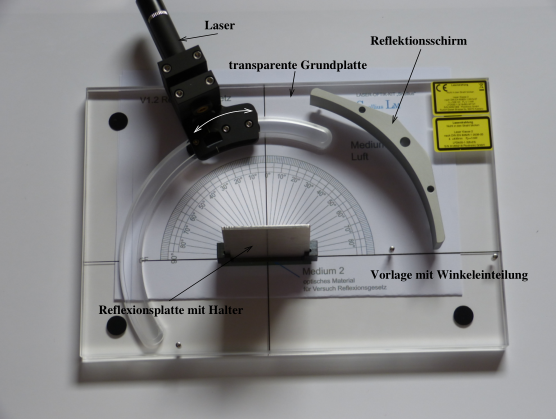
\includegraphics[width=0.35\textwidth]{latex/images/D1.PNG}
            \caption{Ein Bild der Grundplatte.\protect \cite{400}.}
        %    \label{img:schem}
        \end{figure}

        \begin{figure}[H]
            \centering
            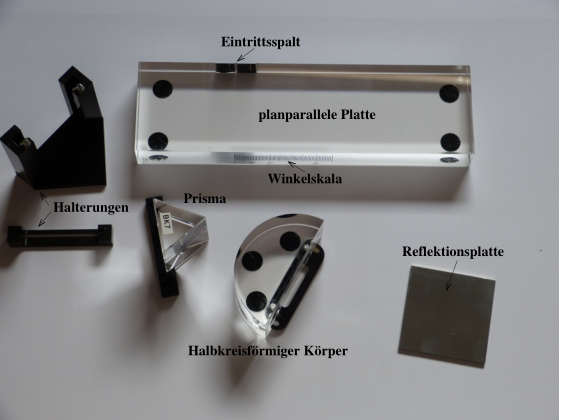
\includegraphics[width=0.35\textwidth]{latex/images/D2.PNG}
            \caption{Ein Bild der unterschiedlichen optischen Elemente\protect \cite{400}.}
            \label{img:object}
        \end{figure}
        
        \noindent
        Bei dem Aufbau der unterschiedlichen Teil-Experimente ist darauf zu achten, dass die optischen Elemente nur an den Halterungen berührt werden, 
        da die Oberfächen sonst beschädigt werden.

    \subsection{Durchführung}

        \textbf{Aufgabe 1}\\

            \noindent
            Für Aufgabe 1 wird auf die Grundplatte ein Spiegel aufgesetzt und für den grünen Laser 7 Messpaare aus Einfallswinkel und Reflexionswinkel
            gemessen.\\

        \textbf{Aufgabe 2}\\
            
            \noindent In Aufgabe 2 wird die planparallele Platte \ref{img:object} aufgesetzt und wieder mit dem grünen Laser 7 Messpare aus dem 
            Einfallswinkel und Brechungeswinkel abelsen. Der Brechungswinkel läst sich innerhalb der planparallele Platte abgelesen.\\
        
        \textbf{Aufgabe 3}\\

            \noindent Für Aufgabe 3 können die Messwerte aus Aufgabe 2 genutzt werden. \\

        \textbf{Aufgabe 4}\\

            \noindent Nun wird die planparallele Platte durch das Prisma ersetzt und die Richtige Vorlage unter die Platte geschoben so, dass der 
            Einfallswinkel und und der Ausfallswinkel aus dem Prisma abgelsen werden können. In diesem Teilversuch werden jeweils 5 Messpaare für den 
            grünen und den roten Laser aufgenommen.\\

        \textbf{Aufgabe 5}\\

            \noindent Zuletzt werden jeweils für die Gitter mit den Gitterkonstanten 600, 300 und 100,  für rotes Licht die Abstände der Maxima zum 
            Mittelpunkt vermessen.\\
        
        